\documentclass{article}
\usepackage{booktabs}
\usepackage{caption} % Include the caption package
\captionsetup{justification=raggedright,singlelinecheck=false}
\usepackage{graphicx}
\usepackage{pgf}


\begin{document}


\title{An example report file from modelflow }
\author{Ib Hansen}
\date{\today} 

% Create the title page
\maketitle
\tableofcontents
\newpage
\section{First a chart} 
Here we se the growth rates in the different scenarios

 
\begin{figure}[htbp]
\centering
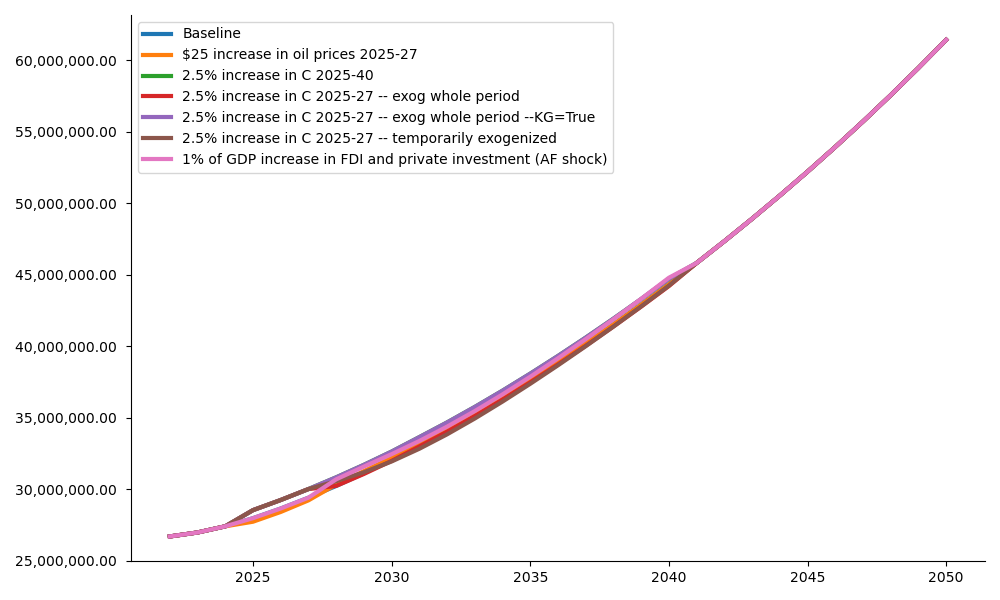
\includegraphics[width=\textwidth]{"../level/Real GDP, level nodif.png"}
\caption{Level: Real GDP}
\end{figure} 
 
\begin{figure}[htbp]
\centering
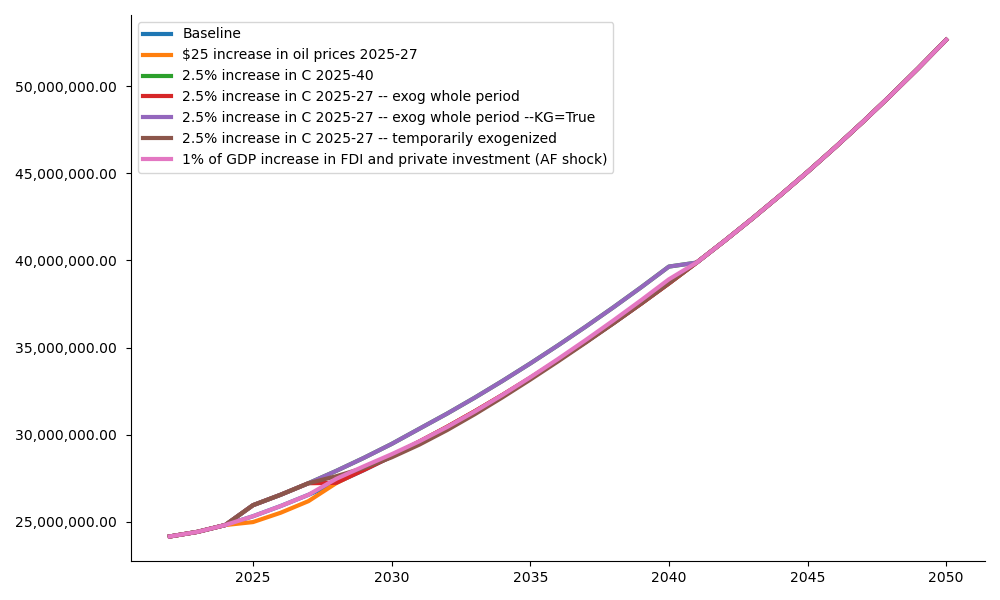
\includegraphics[width=\textwidth]{"../level/HH. Cons Real, level nodif.png"}
\caption{Level: HH. Cons Real}
\end{figure} 
\section{then a chart}
 
\begin{figure}[htbp]
\centering
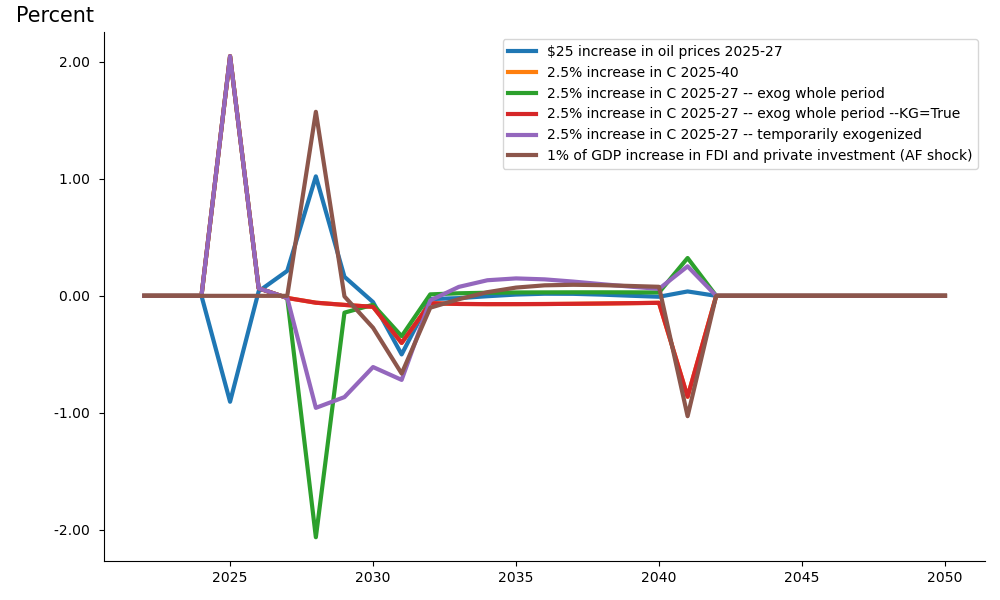
\includegraphics[width=\textwidth]{"../A_plot/Real GDP, growth dif.png"}
\caption{Difference to "Baseline" for Growth: Real GDP}
\end{figure} 
 
\begin{figure}[htbp]
\centering
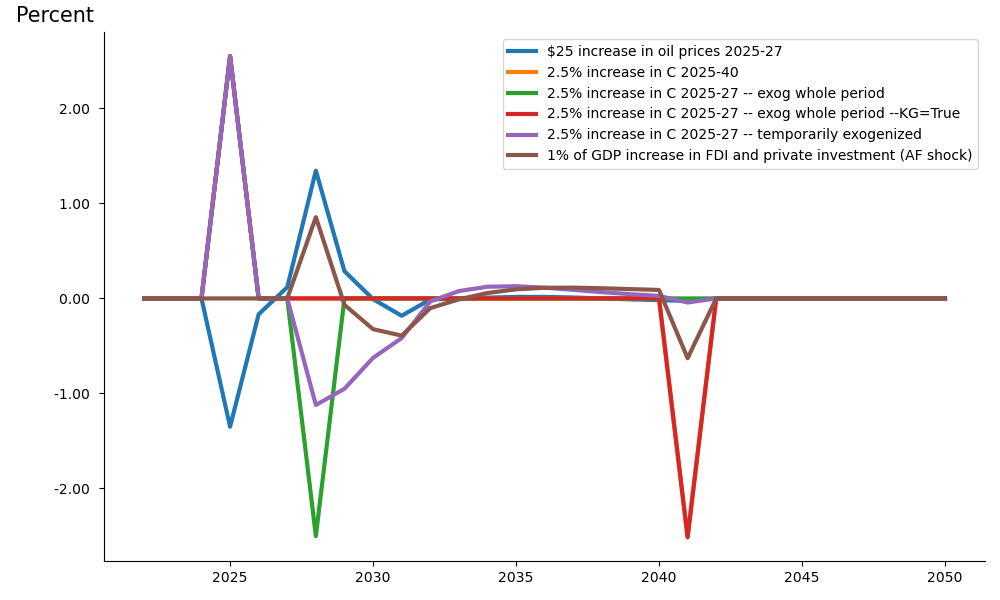
\includegraphics[width=\textwidth]{"../A_plot/HH. Cons Real, growth dif.png"}
\caption{Difference to "Baseline" for Growth: HH. Cons Real}
\end{figure} 
 \section{And a table}
\begin{table}[ht]
\caption{Table}
\begin{tabular}{lrrrrr}
\toprule
 & 2025 & 2026 & 2027 & 2028 & 2029 \\
\midrule
&\multicolumn{5}{c}{{Baseline}}                          \\
&\multicolumn{5}{c}{{--- Percent growth ---}}                          \\
Real GDP & 2.08 & 2.42 & 2.64 & 2.79 & 2.91 \\
HH. Cons Real & 2.03 & 2.32 & 2.48 & 2.59 & 2.69 \\
Investment real & 1.10 & 1.46 & 1.82 & 2.17 & 2.51 \\
Exports real & 4.37 & 4.20 & 4.04 & 3.90 & 3.77 \\
Imports real & 3.10 & 3.10 & 3.02 & 2.89 & 2.78 \\
&\multicolumn{5}{c}{{--- Percent of GDP ---}}                          \\
General Government Revenue, Deficit, LCU mn & -3.05 & -2.98 & -2.95 & -2.92 & -2.91 \\
General government gross debt millions lcu & 57.02 & 57.26 & 57.69 & 58.26 & 58.94 \\
Current Account Balance, US\$ mn & -3.55 & -3.46 & -3.40 & -3.37 & -3.36 \\
&\multicolumn{5}{c}{{Alternative}}                          \\
&\multicolumn{5}{c}{{--- Percent growth ---}}                          \\
Real GDP & 2.08 & 2.42 & 2.64 & 4.36 & 2.91 \\
HH. Cons Real & 2.03 & 2.32 & 2.48 & 3.45 & 2.62 \\
Investment real & 1.10 & 1.46 & 1.82 & 12.46 & 2.98 \\
Exports real & 4.37 & 4.20 & 4.04 & 3.88 & 3.72 \\
Imports real & 3.10 & 3.10 & 3.02 & 4.68 & 2.84 \\
&\multicolumn{5}{c}{{--- Percent of GDP ---}}                          \\
General Government Revenue, Deficit, LCU mn & -3.05 & -2.98 & -2.95 & -2.81 & -2.84 \\
General government gross debt millions lcu & 57.02 & 57.26 & 57.69 & 57.11 & 57.55 \\
Current Account Balance, US\$ mn & -3.55 & -3.46 & -3.40 & -3.48 & -3.43 \\
&\multicolumn{5}{c}{{Impact}}                          \\
&\multicolumn{5}{c}{{--- Impact, Percent growth ---}}                          \\
Real GDP & 0.00 & 0.00 & 0.00 & 1.57 & -0.00 \\
HH. Cons Real & 0.00 & 0.00 & 0.00 & 0.86 & -0.07 \\
Investment real & 0.00 & 0.00 & 0.00 & 10.29 & 0.47 \\
Exports real & -0.00 & -0.00 & -0.00 & -0.02 & -0.05 \\
Imports real & 0.00 & 0.00 & 0.00 & 1.79 & 0.06 \\
&\multicolumn{5}{c}{{--- Impact, Percent of GDP ---}}                          \\
General Government Revenue, Deficit, LCU mn & -0.00 & -0.00 & -0.00 & 0.11 & 0.07 \\
General government gross debt millions lcu & -0.00 & -0.00 & -0.00 & -1.15 & -1.39 \\
Current Account Balance, US\$ mn & 0.00 & -0.00 & -0.00 & -0.11 & -0.06 \\
\bottomrule
\end{tabular}
\end{table}

\begin{table}[ht]
\caption{GDP components}
\begin{tabular}{lrrrrr}
\toprule
 & Real GDP & HH. Cons Real & Investment real & Exports real & Imports real \\
\midrule
&\multicolumn{5}{c}{{--- Percent growth ---}}\\
2022 & 0.66 & 0.80 & 0.70 & 4.71 & 3.00 \\
2023 & 1.04 & 1.09 & 0.63 & 4.66 & 2.86 \\
2024 & 1.60 & 1.60 & 0.79 & 4.53 & 2.99 \\
2025 & 2.08 & 2.03 & 1.10 & 4.37 & 3.10 \\
2026 & 2.42 & 2.32 & 1.46 & 4.20 & 3.10 \\
2027 & 2.64 & 2.48 & 1.82 & 4.04 & 3.02 \\
\bottomrule
\end{tabular}
\caption*{Source: World bank }
\end{table}

\end{document}
        